\documentclass[listof=totoc,bibliography=totocnumbered,a4paper,english,12pt,twoside]{report}

\usepackage{graphicx,caption,subcaption,float}
\usepackage[english, ngerman]{babel,varioref}
\usepackage{svg}
\usepackage[utf8]{inputenc}
\usepackage[T1]{fontenc}
\usepackage{pslatex}
\usepackage{layouts}
\usepackage{tabularx}
\usepackage[separate-uncertainty=true,per-mode=fraction]{siunitx}
\usepackage{isotope}
\usepackage[section]{placeins}
\usepackage{graphicx}
\usepackage{textgreek}
\usepackage{amssymb}
\usepackage{hyperref}
\usepackage{appendix}
\usepackage{acronym}
\usepackage{subcaption}
\usepackage{multirow}
\usepackage{hypdvips}
\usepackage{booktabs}
\usepackage{etoolbox}
\usepackage{longtable}
\usepackage{rotating}
\usepackage[acronym,automake]{glossaries}
\usepackage[nottoc]{tocbibind}
\usepackage{lmodern}
\usepackage{pdfpages}

\usepackage{lscape}
\usepackage{pdflscape}


%% The amsthm package provides extended theorem environments
\usepackage{amsthm}
\usepackage{amsmath}
%% The lineno packages adds line numbers. Start line numbering with
%% \begin{linenumbers}, end it with \end{linenumbers}. Or switch it on
%% for the whole article with \linenumbers.
%\RequirePackage{lineno}\newdimen\linenumbersep\linenumbersep=2pt\linenumbers
%\usepackage{lineno}
\usepackage{color}
\usepackage{printlen}
%\uselengthunit{in}\printlength\textwidth

\usepackage{setspace}

%new SI units
\DeclareSIUnit\adcu{ADCu}
\DeclareSIUnit\pe{p.e.}
\DeclareSIUnit\inch{in}
\DeclareSIUnit\sample{S}
\sisetup{table-align-uncertainty=true,exponent-product = \cdot}

%new svg path
\svgpath{plots/}



\pagestyle{headings}                 % Seitenstil
\oddsidemargin0.8cm                  % linker Rand fuer ungerade Seiten bei \twoside
\evensidemargin0.2cm                 % linker Rand fuer gerade Seiten (nur bei \twoside)
\topmargin0.5cm                      % oberer Rand bis zur Oberseite Kopfzeile
\textheight21cm                      % Texth"ohe auf einer Seite
\textwidth15cm                       % Textbreite auf einer Seite
\renewcommand{\topfraction}{0.75}    % Anteil der Gleitk"asten am Seitenanfang
\renewcommand{\bottomfraction}{0.75} % Anteil der Gleitk"asten am Seitenende
\parskip1ex  plus1ex minus0.5ex      % Abstand zwischen Abs"atzen
\parindent0em                        % Einr"uckung der ersten Zeile eines Absatzes
\newcommand{\clearemptydoublepage}{\newpage{\pagestyle{empty}\cleardoublepage}}

\begin{document}
\onehalfspacing
\begin{titlepage}
\newcommand{\HRule}{\rule{\linewidth}{0.25mm}} % Defines a new command for the horizontal lines, change thickness here
\center
\textsc{\LARGE Albert-Ludwigs-Universit\"{a}t Freiburg}\\[1.5cm]
\textsc{\Large Master Thesis}\\[0.4cm]
\HRule \\[0.4cm]
{\huge \bfseries Readout of a five dimensional} \\[0.2cm] 
{\huge \bfseries Calorimeter} \\[0.2cm]
%{\huge \bfseries small- to medium-size experiments} 
\\[0.2cm]
\HRule \\[1.5cm]

\begin{minipage}{0.4\textwidth}
\begin{flushleft} \large
\emph{Author:}\\
Johannes \textsc{Alt} \\
\end{flushleft}
\end{minipage}
~
\begin{minipage}{0.4\textwidth}
\begin{flushright} \large
\emph{Supervisor:} \\
Prof. Dr. Horst \textsc{Fischer} \\
\end{flushright}
\end{minipage}\\[2cm]

{\large June 20, 2022}\\[1cm]


\includegraphics[width=5cm, keepaspectratio]{pictures/siegel.png}\\[1cm]

\large \emph{Fakult\"{a}t f\"{u}r Mathematik und Physik}\\[0.4cm]

\HRule \\
\setcounter{page}{0}
\end{titlepage}





\newpage
\thispagestyle{empty}
\mbox{}\newpage
\selectlanguage{english}
\begin{abstract}
    The SHiP experiment is planned to be a zero background beam dump experiment at the CERN's SPS accelerator. To achieve the zero background goal, the SBT is under development to tag all background events. It is a five-dimensional tagger based on a liquid scintillator. The scintillation light caused by particles traveling through the scintillator is captured by WOMs and detected by SiPMs. This thesis is in the framework of R\&D of these SiPMs. Therefore the Citiroc 1A ASIC was used and tested with a array of 40 SiPMs. Using the Citiroc 1A evaluation board for a compact and easy to use DAQ measurements with the SiPMs in darkness as well as with a controlled light exposure via a LED and a Laser were performed. Also the effects of up to five SiPMs connected in parallel were analysed.
    A calibration of one SiPM and up to five SiPMs in parallel was performed as well as a measurement of the dark count rate.
\end{abstract}
\thispagestyle{empty}
\mbox{}\newpage
\thispagestyle{empty}
\selectlanguage{ngerman} 

\begin{abstract}
	\setcounter{page}{3}  
	asdf
\end{abstract}
\selectlanguage{english}


\thispagestyle{empty}
\newpage
\thispagestyle{empty}
\mbox{}\newpage

\pagenumbering{arabic}
\setcounter{page}{1}
\tableofcontents

\newpage
%\chapter{Introduction}

\begin{itemize}
    \item SM
    \itme 
\end{itemize}




\chapter{Motivation}

\begin{itemize}
    \item SHiP
    \itme 
\end{itemize}



\chapter{Calorimeter}

\begin{itemize}
    \item 
\end{itemize}



\chapter{Setup}

\section{Citiroc 1A}

\begin{itemize}
    \item overview with sketch
    \item input dac
    \item IN\_CALIB
    \item amplifier
    \item trigger
    \begin{itemize}
        \item fast shaper
        \item threshold dacs (10 bit and 4 bit)
        \item discriminator 
        \item charge trigger
        \begin{itemize}
            \item masking capabilities
            \item multiplexer
            \item OR32\_charge and OR32\_charge\_OC
        \end{itemize}
        \item time trigger
        \begin{itemize}
            \item 32 outputs
            \item OR32\_charge\_OC
        \end{itemize}
    \end{itemize}
    \item Charge measurement
    \begin{itemize}
        \item shaper
        \item peak sensing
        \begin{itemize}
            \item SCA
            \begin{itemize}
                \item constant tracking of shaper output
                \item external hold on high level
                \item holding of shaper amplitude while hold on high
                \item multiplexer
                \item hold on low level: return to tracking
            \end{itemize}
            \item peak detector
            \begin{itemize}
                \item idle mode
                \item external trigger or internal charge trigger
                \item starts tracking the maximum of the shaper output
                \item external hold on high level
                \item holding maximum amplitude until
                \item multiplexer
                \item hold on low level: return to idle 
            \end{itemize}
        \end{itemize}
        \item multiplexer
    \end{itemize}
    \item probing
    \item temperature sensor
\end{itemize}

\section{Citiroc 1A Evaluation Board}

\begin{itemize}
    \item Citiroc 1A
    \item 32 inputs
    \item In\_calib
    \item probe outputs
    \item ADCs
    \item FPGA
    \item usb interface
    \item power supply
    \item HV
    \item Software
    \begin{itemize}
        \item slow control
        \item hold scan
        \item measurement
    \end{itemize}
\end{itemize}



\section{SiPM array}


\section{light source}
\begin{itemize}
    \item LED
    \begin{itemize}
        \item wavelength
        \item waveform generator settings
    \end{itemize}
    \item diffusor 
\end{itemize}

\section{Box}


\chapter{Measurements}
\begin{itemize}
    \item first linearity test
    \item dark count measurements
    \begin{itemize}
        \item dark count rate
        \item gain
    \end{itemize}
    \item 
\end{itemize}
\subsection{Waveform generator measurement}
\begin{itemize}
    \item goal: linearity.
    \item setup: wfgenerator, attenuator and voltage-to-charge
    \item charge signal per \SI{50}{\milli\volt}
    \item how/what measurement was performed
    \item start with 50mV, and increase voltage
    \item histogram
    \item plot: mean output over input
    \item linear to which channel
\end{itemize}

\section{Dark count measurement}

\subsection{dark count rate}

\subsection{dark count gain/calibration}


\section{Measurement with light source}



\chapter{Conclusion and Outlook}


\begin{itemize}
    \item 
\end{itemize}
\chapter{Introduction}
The \ac{sm} provides the best description of the universe.
But through observations of different phenomena, which the \ac{sm} can not explain, like neutrino oscillation \cite{} and the rotation velocity in galaxies \cite{}, it is known, that the \ac{sm} can not be a complete theory \cite{}.
Therefore different experiments are in developement or are operating to search for new physics and new particles outside the \ac{sm}.
One of these experiments is the proposed \ac{ship} experiment.
Some experiments are at the energy frontier, using large energy scale trying to discover new particles. The experiments at the \ac{lhc} are examples for energy frontier experiments.
Other experiments are at the cosmic frontieri, using for example cosmic background radiation.
The third frontier is the intensity frontier.
The zero background \ac{ship} experiment is one of the intensity frontier experiment searching for rare events.
Observing such rare events requires a high interaction rate.
To achieve this, \ac{ship} is planned to be a beam dump experiment at the \ac{sps} accelerator ring at CERN, as shown in \autoref{fig:sps_ship}.
The goal is to dump the high intensity \SI{400}{\giga\electronvolt} proton beam into a fixed target and thereby creating long lived particles outisde of the \ac{sm}, e.g. heavy neutral leptons and light supersymmetric particles \cite{ship}.
\begin{figure}
	\centering
	\includegraphics[width=0.75\textwidth]{pictures/ship_sps}
	\caption[Plan of the SPS area in which SHiP is supposed to be build.]{An overview of the SPS area with the SHiP experiment planed as beam dump experiment in the north area. \cite{ship_facility}}
	\label{fig:sps_ship}
\end{figure}

In \autoref{fig:ship_sketch} the overall struckture of \ac{ship} is shown.
At the beginning, the \SI{400}{\giga\electronvolt} gets dumped into the fixed targed.
Through the many interactions happening at the target, a lot of \ac{sm} particles will be created.
In order to block the \ac{sm} particles, two shields are placed after the target.
The first is a hadron absorber in which all \ac{sm} particles except muons and neutrinos are absorbed.
The second is the muon shield. 
It uses magnetic fields to deflect the muons away from the beam line.
The neutrinos cannot be blocked or deflected, but they are likely to be detected in the scattering and neutrino detector behind the muon shield.
After the neutrino detector a \SI{50}{\meter} long vacuum chamber is positioned.
If a non \ac{sm} particle is created at the target, is can decay inside the vacuum decay chamber back into \ac{sm} particles.
The decay products than get measured in the decay spectrometer behind the decay chamber.

One problem for the measurement are \ac{sm} particles entering the decay volume and causing events in the spectrometer.
An example of such a background are muons deflected by the muon shield but afterwrads reflected by the walls of the facility into to decay volume.
Therefore it is crucial for the zero background requirment to detect the particles entering the decay volume and tagging every event that could be caused by the entering particle as background.
For this the \ac{sbt} is in developement.
It is presented in the next chapter.



\begin{figure}
	\centering
	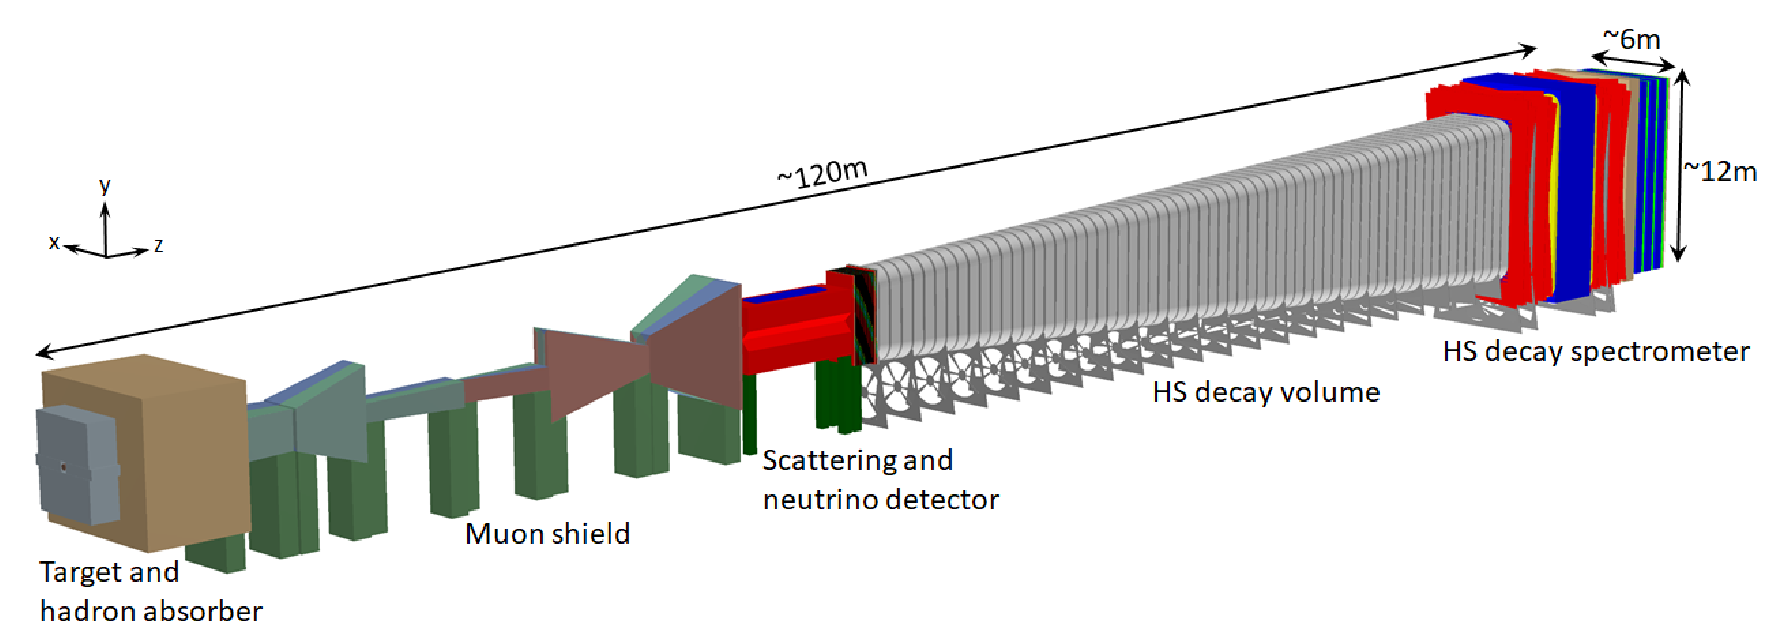
\includegraphics[width=1.\textwidth]{pictures/ship_sketch}
	\caption[Overview of the SHiP experiment.]{Overview of the proposed setup for the SHiP experiment. The target on the left is used as a beam dump for the SPS. Most standard model particles get absorbed by the hadron absorber directly behind the targed. A magnetic muon shield deflects the muon, which won't be absorbed by the hadron absorber, away from the beam line. After the muon shield is a scattering and neutrino detector and afterwards the \SI{50}{\meter} long decay volume in which non standard model particles created at the target can decay into standard model particles. To achieve the zero background goal, the Sourrund Background Tagger is around the decay volume. Behind the decay volume the decay spectrometer is placed. \cite{ship_coll}}
	\label{fig:ship_sketch}
\end{figure}

%\chapter{The SBT as 5 Dimensional Calorimeter}
For the \ac{sbt} to allow the tagging of background events, it needs to provide multiple pieces of information about the measured events and therefore the particles entering the decay volume. 
To achieve this, the \ac{sbt} is designed to be a five-dimensional tagger around the decay volume. 
It consists out of 2000 cells, each filled with with the liquid scintillator \ac{lab}.
If a particle passes through the cell, it deposits energy in it, causing the emittance of scintillation light.
The amount of scintillation light is proportional to the deposited energy and therefore it depends on the energy of the particle, the interaction crosssection of the particle and the length of the path inside the cell that the particle traveled.
Each cell houses two \acp{wom}.
If the scintillation light enters a \ac{wom}, the wavelength get shifted and through total reflection the photons stay in the \ac{wom} until they reache the end of the \ac{wom} tube.
There they get detected by an array of photosensors. 
The concept of the cells, scintillator, \acp{wom} and photosensor is depicted in \autoref{fig:sbt_cell}
By comparing the amount of light detected in each of the two \acp{wom} one can estimate roughly the path of the particle.
Adding this information to the information in which of the cells the particle was detected, the three spacial dimensions of the particle entering the \ac{sbt} are known.
Also by the detected amount of light, the energy as fourth dimension can be measured.
The fifth dimension is the timing of the event. 
By using Silicon Photomultiplier as photosensor, a good time resolution can be achieved.

This thesis is about the readout of these Silicon Photomultipliers and therefore they are presented in this chapter with more detail.

\begin{figure}
	\centering
	\includegraphics[width=1.\textwidth]{pictures/sbt_cell}
	\caption[Overview of the SBT]{Overview of the functionality of the Surround Background Tagger consisting out of 2000 cells. The cells are filled with liquid scintillator and are housing two Wavelength-shifting Optical Modules which capture the scintillation light and guide it to the Silicon Photomultipliers mounted at one and of the WOM. \cite{bsc_jonathan}}
	\label{fig:sbt_cell}
\end{figure}



\section{Silicon Photomultiplier}
In order to correctly identify and tag background events, the light detection of the \ac{sbt} has to provide accurate timing information.
Therefore \acp{sipm} were chosen as photodetectors.
These photodetectors consist of up to thousands of pixels.
Each pixel is a photodiode with a typical edge length between \SI{10}{\micro\meter} and \SI{100}{\micro\meter} \cite{nucl}.
If triggered by light, a \ac{sipm} sends out a charge signal proportional to the incoming light.
This charge possesses a fast-rising edge with a rise time of the order of tens of \si{\piko\second} \cite{nucl}.
Besides the good time resolution, \acp{sipm} also make it possible to count the arriving photos with a sensitivity down to single photons \cite{HAMA_mppc}.


Similar to every photodiode, \acp{apd} utilize the photoelectric effect, to generate an electric charge signal in response to a light signal.
This is made possible by using silicon as a base material and introducing impurities. 
This process is called doping and there are two different possibilities for doping. 
In the n-doping, the impurities are atoms with five valence electrons.
Four of these electrons are part of boundings with silicon atoms, and the fifth electron is only weakly bound.
When p-doping, atoms with only three valence electrons are inserted into the silicon.
This leads to missing charges in the silicon, called holes.
By having an n-doped and a p-doped region in the silicon, the excess electrons from the n-doped region combine with the holes from the p-doped region, resulting in a depleted region at the pn-junction.
If a photon hits the photodiode, it can create an electron-hole pair, or $eh$-pair.
The electron and the hole get split by the electric field and thus create a charge signal.
In order to increase the sensitivity of the photodiode, an intrinsic layer can be added in between the two doped regions, thus increasing the depletion layer and therefore the photosensitive area.
Such a photodiode is called a pin-diode.
An \ac{apd} with a weakly doped $\pi$ intrinsic layer and strongly doped $p^+$ and $n^+$ layers is shown in \autoref{fig:pin_diode}.
This intrinsic layer can either be not doped at all or weakly doped.
In the case of \acp{apd} the intrinsic layer is weakly doped. 
In order to amplify the signal, a strong doped region is inserted, thus creating a multiplication zone.
\begin{figure}
	\centering
	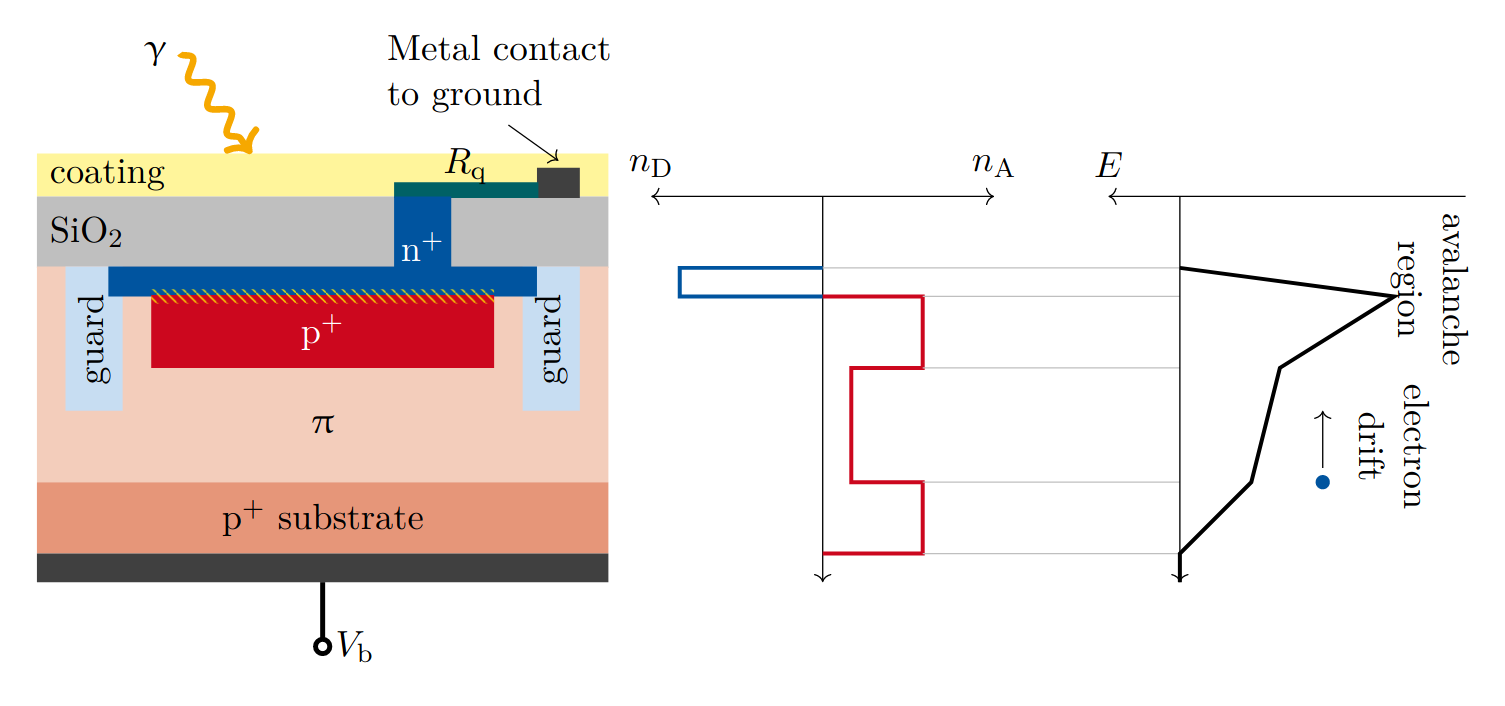
\includegraphics[width=1.\textwidth]{pictures/pin_diode}
	\caption[Illustration of a APD.]{Composition of a avalanche photo diode with the bias voltage $V_\text{B}$ applied in reverse direction. Between the contact to ground and the strongly doped $n^+$ layer is the quenching resistor $R_\text{q}$ connected in series. Next to the $n^+$ layer is a strongly doped $p^+$ layer. In the region of these two layers is the electric field, shown on the right figure, the strongest. There a electron or hole can initiate an avalanche. After the $p^+$ layer comes a intrinsic weakly doped $\pi$ layer. This layer increases the sensitive volume of the diode. If a electron-hole pair is created and seperated by the electric field. The hole drifts towards the multiplication region and can start an avalanche. The next layer is a $p^+$ layer which connects to a metal connector and high voltage. \cite{kemp}}
	\label{fig:pin_diode}
\end{figure}

When a reverse bias voltage is applied to the \ac{apd}, the electric field between the $n^+$ and $p^+$ layers is strong enough that a created $eh$-pair creates more $eh$-pairs, resulting in an avalanche.
For this avalanche process to be possible the reverse bias voltage must be at or above the breakdown voltage of the \ac{apd}.
With such a bias voltage applied, the \ac{apd} operates in the Geiger mode and the avalanche is then self-sustaining.
This results in a macroscopic signal and makes the detection of single photons possible.
Therefore these diodes are also called \ac{spad}.
To stop the avalanche, a quenching resistor is connected in series with the \ac{spad}.
With an increasing current signal flowing through the quenching resistor, the voltage drop at this resistor increases, and thus the bias voltage at the \ac{spad} decreases.
When the bias voltage drops under the breakdown voltage, the avalanche is no longer self-sustaining and stops.
Thus the signal amplitude of a \ac{spad} is always similar, independent of how many photons arrive at the same moment.
In \acp{sipm} hundreds to thousand \acp{spad} are connected in parallel, each with a high resistance quenching resistor in series. 
Usually, the \ac{spad} pixels are placed in a rectangular form with an edge length of a few \si{\milli\meter}.
\autoref{fig:sipm_closeup} shows a picture of a \ac{sipm} and one picture of a single pixel of a \ac{sipm}.
Due to the property of the \acp{spad} that the output signal is always similar for each \ac{spad}, the output signal of a \ac{sipm} is the output signal of one \ac{spad} multiplicated with the number of triggered \acp{spad}.
Therefore, if the number of photons arriving simultaneously at a \ac{sipm} is low enough, that the probability of one \ac{spad} being hit by two or more photons is low, one can count photons with a \ac{sipm}.
This and the relatively low cost, high durability, and impassivity to magnetic fields make them a good option for photodetection for the \ac{sbt} and similar detectors.

In the following different properties of \acp{sipm} are presented, beginning with the signal shape of a single \ac{spad} and of a \ac{sipm}.


\paragraph{The signal shape} of a \acp{spad} starts with a fast exponential rise with the time constant 
\begin{align}
	\tau_\text{rise}&=R_\text{S}\cdot C_\text{d}
\end{align}
with the resistance $R_\text{rise}$ and capacitance $C_\text{d}$ of the \ac{spad} \cite{HAMA_mppc}.
After the signal reached its maximum current at around 
\begin{align}
	I_\text{max}&\approx \frac{V_\text{ov}}{R_\text{q}}
\end{align}
the quenching and recharging of the \ac{spad} starts.
Thus the current signal decreases again exponentially.
The time constant for the signal decay
\begin{align}
	\tau_\text{decay} &= R_\text{q}\cdot C_\text{d}
\end{align}
depends on the capacitance $C_\text{d}$ of the \ac{spad} and the quenching resistor $R_\text{q}$ \cite{HAMA_mppc}.
This signal develpment is shown in \autoref{fig:spad_signal_shape}.
\begin{figure}
	\centering
	\includegraphics[width=0.75\textwidth]{pictures/spad_signal_shape}
	\caption[SPAD signal shape]{Single photon avalanche diode signal shape. The exponential rise with the time constant $R_\text{S}\cdot C_\text{d}$ is followed by the exponential decay with the time constants $R_\text{q}\cdot C_\text{d}$. The maximum of the current signal is at approximately $V_\text{ov}/R_\text{q}$ \cite{HAMA_mppc}}
	\label{fig:spad_signal_shape}
\end{figure}

When multiple \acp{spad} in a \ac{sipm} are triggered, the output signal will be the summation of the signals from all triggered \acp{spad}.
Besides the number of triggered \acp{spad}, the time difference between the signals from the single \acp{spad} influences the signal.
In the case, that all \acp{spad} are triggered at the same time, the \ac{sipm} signal will have the shape of a \ac{spad} signal scaled up by the factor of the number of triggered \acp{spad}.
If the signals form the individual \acp{spad} have a small difference in time, the \ac{sipm} signal will become broader.




\paragraph{The gain} $G$ of a \ac{sipm} describes the number of charge carriers released in each avalanche.
Due to the quenching, this parameter is well defined \cite{}.
It can be calculated from the applied voltage $U_\text{bias}$, the breakdown voltage $U_\text{bd}$ and the capacitance $C_\text{d}$ of a \ac{spad} with
\begin{align}
	G &= \frac{(V_\text{bias}- V_\text{bd})\cdot C_\text{d}}{\text{e}}.
\end{align}
Here e represents the charge of one electron.
Usually the gain is in the order of $10^5$ to $10^7$ \cite{nucl}.

\paragraph{The noise} in \acp{sipm} can be sorted into two categories.
The first is primary noise, it describes the triggering of avalanches by thermaly created $eh$-pairs and not by incident photons.
Because the rate of theses thermaly caused events increases and decreases with the temperature, by controling the temperatur one can influence and decrease the rate of primary noise events.
The second category is the correlated noise.
It includes all events triggered by a primary event.
This correlated noise does have two causes.
One cause is the trapping and releasing of charge carriers from the avalanche. 
When the time between the trapping and releasing is long enough, the avalanche of the primary event stoped and the released carrier can trigger another avalanche.



\subsection{Photoelectron spectrum}


After the theory and important properties of \acp{sipm} are now introduced, the next chapter will present the measurement setup and data acquisition used for this thesis.

%\chapter{Setup}
In this chapter, the setup and its components are introduced. 
First, the Citiroc 1A \ac{asic} and its evaluation board are presented. 
Then the used \ac{sipm} array is shown and in the last part of this chapter the box housing the \ac{sipm}s during the measurements is presented.



\section{Citiroc 1A}
Developed by the company Weeroc, the Citiroc 1A is an \ac{asic} for the readout of \ac{sipm}s. 
In essence, it is an amplifier and shaper for an input signal with trigger capabilities and a multiplexer output for the shaper signal amplitude.
So the charge signal coming from a \ac{sipm} gets amplified by the amplifier and integrated by the shaper.
The maximum of this integrated signal is than connected to a multiplexed output.
With this multiplexed output, all channels can be read out one after another at the same output of the Citiroc 1A.
Therefore the number of \acp{adc} needed to digitize the signals from every channel is reduced by a factor of 31.
A sketch of the internal electronics of the Citiroc 1A is shown in \autoref{fig:citiroc1a_sketch}.

\begin{figure}
    \centering
    \includegraphics[width=1.\textwidth]{citiroc/citiroc}
    \caption[Citiroc 1A sketch]{Depiction of the main components of the Citiroc 1A. 
	The 32 channels with the inputs and the input DACs are followed by a low and a high gain preamplifier. 
	Both amplified signals are shaped by slow shapers and the peak sensing cell returns the shaper signal amplitude to a multiplexer common to all channels. 
	Also, the trigger part with a fast shaper followed by two discriminators is shown. 
	One discriminator output is connected to a common multiplexer and an OR of the 32 channels. 
	The other discriminator is connected to a channel by channel time trigger output and also to a common OR. 
	The trigger threshold of both discriminators can be set individually but common for all channels via a 10-bit DAC. \cite{citiroc}}
    \label{fig:citiroc1a_sketch}
\end{figure}

The Citiroc 1A has 32 channels. 
Each channel has an 8-bit input \ac{dac} which allows tuning the high voltage on a channel by channel level.
When the high voltage $V_\text{HV}$ is supplied to the \ac{sipm}s and the \ac{dac} voltage is $V_\text{DAC}$ the bias voltage on the \ac{sipm}s is
\begin{align}
	V_\text{bias} &= V_\text{HV} - V_\text{DAC}.
\end{align}
The input \ac{dac}s are connected to the inputs with resistors in series, so that the fast charge signal from the \ac{sipm}s is not disturbed by the input \ac{dac}.
Besides the 32 inputs, one \textit{IN\_CALIB} input exists with which a signal can be injected into one of the 32 channels.
The injected signal goes over a \SI{3}{\piko\farad} capacitor into the preamplifier.
A sketch of this is shown in \autoref{fig:citiroc_amp}.
After the input, there are two amplifiers in parallel.
One high gain amplifier and one low gain amplifier so that a broader input range can be covered.
The structure of both amplifiers is the same and shown in \autoref{fig:citiroc_amp}.
They each have a capacitor $\text{C}_\text{in}$ in series and then a variable feedback capacitor $\text{C}_\text{f}$ in parallel, which can be set to values from \SIrange{0}{1575}{\femto\farad} in \SI{25}{\femto\farad} steps.
The capacitors connected in series have fixed capacitances.
The low gain preamplifier capacitor has \SI{1.5}{\piko\farad} and the high gain preamplifier has a \SI{15}{\piko\farad} capacitance.
The Citiroc 1A datasheet states that the resulting amplification can be calculated with
\begin{align}
	AMP &= \frac{\text{C}_\text{in}}{\text{C}_\text{f}}.
\end{align}
Since this equation is not defined for $\text{C}_\text{f}=\SI{0}{\femto\farad}$, that value was not used for the measurements in this thesis.
For the other possible feedback capacitor values the resulting high gain and low gain amplifications are \SIrange[per-mode=symbol]{9.5}{60}{\volt\per\volt} and \SIrange[per-mode=symbol]{0.95}{6}{\volt\per\volt}, respectively. 
Each amplifier output is connected to a slow shaper and in addition one of the outputs can be connected to the trigger block of the Citiroc 1A.

\begin{figure}
	\centering
	\includegraphics[width=0.5\textwidth]{citiroc/preamp}
	\caption[Sketch of the Citiroc 1As preamplifiers]{Illustration of the preamplifiers in the Citiroc 1A. The signal is injected either through the IN input or through the IN\_Calib input. By changing the capacitance of the feedback capacitor, the gain can be set. \cite{citiroc}}
	\label{fig:citiroc_amp}
\end{figure}


\paragraph{The trigger unit} starts with the shaping of the amplifier output connected to the trigger unit. 
This is done by a CRRC fast shaper with a \SI{15}{\nano\second} peaking time \cite{citiroc}. 
The high pass filter of the fast shaper consists of a $C_\text{in}=\SI{5}{\piko\farad}$ capacitor and a $R_\text{in}=\SI{500}{\ohm}$ resistor.
The low pass filter constists of a $C_\text{f}=\SI{100}{\femto\farad}$ capacitor and a $R_\text{f}=\SI{25}{\kilo\ohm}$ resistor.
In \autoref{fig:fast_shaper} the schematics of the fast shaper are shown.
After the shaping, the signal goes into two discriminators.
By using the two 10-bit \ac{dac}s and the 4-bit \ac{dac}s, also connected to the discriminator, a trigger threshold can be set.
While the two 10-bit \ac{dac}s are common for all the 32 channels, each channel has its own two 4-bit \ac{dac}s.
This allows to fine-tune the common threshold set by the 10-bit \ac{dac}s on a channel by channel level.
The time discriminator output is connected to an open-collector NOR of all 32 channels and can also be read out channel by channel, enabling the setting of time stamps for each channel.
The charge discriminator is followed by masking opting, which allows the channel by channel masking of the charge trigger. 
After the masking option, the charge trigger signal is connected to an OR of the 32 channels which can be read out as an OR or as an open-collector NOR.
The charge trigger can also be connected to a multiplexed output of all channels.
With this output, one can easily see in the measurement data which channel was triggered in each event.
Both triggers are sensitive down to 1/3 of a photoelectron \cite{citiroc}.

\begin{figure}
	\centering
	\includegraphics[width=.5\textwidth]{citiroc/fast_shaper}
	\caption[Citiroc 1A fast shaper schematic]{The fast shaper of the Citiroc 1A with the $\SI{5}{\piko\farad}$ capacitor $\text{C}_\text{in}$ and the $\SI{500}{\ohm}$ resistor $\text{R}_\txt{in}$ functioning as high pass filter. The capacitor $\text{C}_\text{f}=\SI{100}{\femto\farad}$ and the resistor $\text{R}_\text{f}=\SI{25}{\kilo\ohm}$ working as a low pass filter. The resulting peaking time is $t_\test{peak}=\SI{15}{\nano\second}$. \cite{citiroc}}
	\label{fig:fast_shaper}
\end{figure}


\paragraph{For the charge measurement} the outputs of the two preamplifiers are connected to two CRRC$^2$ slow shapers, depicted in \autoref{fig:slow_shaper}.
The time constant for the high pass filter and the two low pass filters can be set from \SIrange{12.5}{87.5}{\nano\second} in \SI{12.5}{\nano\second} steps.
This results in an overall peaking time of \SIrange{25}{175}{\nano\second} in \SI{25}{\nano\second}.
\begin{figure}
	\centering
	\includegraphics[width=1.\textwidth]{citiroc/slow_shaper}
	\caption[Citiroc 1A slow shaper schematic]{Schematic of the Citiroc 1As CRRC$^2$ slow shapers. Each CR or RC part has a time constant changeable from \SIrange{12.5}{87.5}{\nano\second} in \SI{12.5}{\nano\second} by changing the capacitance of the capacitors. \cite{citiroc}}
	\label{fig:slow_shaper}
\end{figure}
The slow shapers are followed by a peak sensing cell which gives the maximum shaper amplitude out to a multiplexer.
Two options for finding the amplitude to put out are built in the peak sensing cell.
The first option is the \textit{SCA} which works with the \textit{sample and hold} method.
It recuires an external \testit{hold} signal.
The SCA tracks the shaper output constantly, until the external hold signal rises from low to high.
On the rising edge of the hold signal, it samples the shaper amplitude and holds it until the hold signal falls back to low.
In order to sample the maximum of the shaper amplitude, the rising edge of the hold signal must arrive, when the shaper signal is at its maximum. 


The second peak sensing option is the \textit{peak detector}.
It starts in an idle phase and upon an arriving trigger, the internal charge trigger or an external trigger, it starts tracking the maximum of the shaper amplitude.
When the external hold signal rises to high, the maximum amplitude is held, as long as the hold signal is high.
During that time, the amplitude can be read out via the multiplexer.
When the hold signal falls back to low, the peak detector enters the idle phase again.

The trigger starting the peak sensing tracking phase as well as the hold signal required for the peak sensing and the SCA are both common to all 32 channels.
While the amplitudes of all channels are held, the three multiplexers put out the low gain amplitude, the high gain amplitude, and the charge trigger, one channel after another.
The multiplexer requires an external clock signal to shift between the channels. 
In order to achieve a 10-bit resolution on the output, the clock's frequency should be less than \SI{5}{\mega\hertz}.
This leads to a readout time per channel of at least \SI{200}{\nano\second} and a total readout time of more than \SI{6.4}{\micro\second}.
Since the Citiroc 1A holds the shaper amplitude during that time, it is blind to other events happening while the read-out of the multiplexed output is going on.
Therefore a continuous readout is not possible with the Citiroc 1A.


In order to simplify working with the Citiroc 1A and getting to know it, the Citiroc 1A evaluation board was used.
It is presented in the following section.








\subsection{Citiroc 1A evaluation board}

To make it easier to work with the Citiroc 1A, the corresponding evaluation board houses everything necessary except a computer to operate the Citiroc 1A.
A picture of the Citiroc 1A evaluation board is shown in \autoref{fig:citiroc_evaluation_board}.
In the center of the evaluation board is the Citiroc 1A \ac{asic} placed.
Next to it are 32 pairs of pins for connecting the \ac{sipm}s.
One row is connected to the 32 inputs of the Citiroc 1A and the other one can be used to supply the \ac{sipm}s via the evaluation board with high voltage.
For this purpose, a connector can be soldered on the evaluation board over which the board can be supplied with the high voltage for the \ac{sipm}s.
Over an SMA connector signals can be injected into the Citiroc 1As IN\_CALIB input.
Via three SMA connectors, the analog probes of the Citiroc 1A can be read out.
With two onboard 12-bit \ac{adc}s to read out the low gain and high gain multiplexer outputs of the Citiroc 1A.
Optional one of the \ac{adc}s can be used to digitize a test signal which can be injected into the \ac{adc} over a connector on the evaluation board.
The other \ac{adc} can also be used to read out the temperature probe in the Citiroc 1A.
For processing the digitized measurement data an FPGA is placed on the evaluation board.
The firmware for the FPGA as well as the slow control parameters for the Citiroc 1A can be provided via the USB interface.
This interface can also be used to supply the evaluation board with power instead of using the power connector on the board.
In order to operate the Citiroc 1A evaluation board, Weeroc developed a computer program for the Windows operating system.
With this program, the Citiroc 1A slow control parameter can be chosen and sent to the \ac{asic} as well as some FPGA settings.
The most important FPGA settings are the trigger settings, meaning which signal from the trigger block of the Citiroc 1A is used to trigger an event and the time delay between the arrival of the trigger signal and the sending of the hold signal for the peak sensing cell.

The evaluation board also provides multiple FPGA input/outputs.
With these, for example, the digital trigger signal can be read out or a clock on the evaluation board can be put out and connected as a trigger to a light source.


In the following section, the \ac{sipm} array which was read out with the Citiroc 1A evaluation board is presented. 



%Since, due to ground loops, an external power supply introduced a lot of noise into the measurements, a Laptop was used to supply the power via the USB interface. 
%This laptop was also used for loading the slow control and the FPGA firmware onto the evaluation board and storing the measurement data.
%One FPGA input/output can be used to probe the digital outputs, e.g. the OR trigger of a single channel, of the Citiroc 1A.

\begin{figure}
    \centering
    \includegraphics[width=1.\textwidth]{citiroc/citiroc_evaluation_board.jpg}
    \caption{The Citiroc 1A evaluation board with the Citiroc 1A \ac{asic}, the 32 input pins, the probe outputs, two \ac{adc}s, one FPGA with its input/output connectors, and the USB interface.}
    \label{fig:citiroc_evaluation_board}
\end{figure}










\section{Silicon Photomultiplier Array}
The \ac{sipm} array that was used for the measurements consists of forty \textit{Hamamtsu S14160-3050HS} \ac{sipm}s which were soldered in a circle onto the \ac{pcb} shown in \autoref{fig:hamamatsu_pcb_front} and \autoref{fig:hamamatsu_pcb_back}.
In \autoref{tab:sipm_specs} are the specifications of these \ac{sipm}s listed.
The \ac{sipm}s were placed in a \SI{6}{\centi\meter} outer diameter circle onto the \ac{pcb}.
The connections on the \ac{pcb} were made so that the \ac{sipm}s are connected parallel in groups of five.
Each group has a dip switch with five switches placed between the \ac{sipm}s and the high voltage.
Therefore every individual \ac{sipm} can be turned on and off, simplifying debugging and allowing the examination of the signal difference between different numbers of \ac{sipm}s in parallel.
The circuit diagram of one example \ac{sipm} group is shown in \autoref{fig:hamamatsu_pcb_circuit}. 

\begin{figure}
	\centering
	\includegraphics[width=0.5\textwidth]{pictures/sipm_pcb}
	\caption[Circuit diagram of the connections on the \ac{sipm} \ac{pcb}]{Circuit diagram of the connections on the \ac{sipm} \ac{pcb} for one group of five \acp{sipm}. Each \ac{sipm} can be disconnected from the high voltage via a switch. The high voltage side of the \acp{sipm} is connected to ground over a \SI{100}{\nano\farad} capacitor.}
	\label{fig:hamamatsu_pcb_circuit}
\end{figure}

In order to connect the \ac{sipm} outputs to the Citiroc 1A evaluation board inputs and to supply the \ac{sipm}s with high voltage, a breakout board was used.
It can be connected to the back of the \ac{sipm} \ac{pcb}.
On the back of the breakout board are eight SMA connectors for the signal output of eight \ac{sipm} groups and one SMA connector for the common high voltage supply.
A picture of the breakout board is shown in \autoref{fig:hamamatsu_breakout}.



In order to be able to control the light exposure of the \ac{sipm}s during the measurements, they were placed inside of a light-tight box, which is described in the following chapter.

\begin{figure}
    \centering
    \begin{subfigure}[t]{0.33\textwidth}
        \centering
        \includegraphics[width=.95\linewidth]{pictures/hamamatsu_sipm_pcb_front.jpg}
        \caption{The \ac{pcb} front of the \ac{pcb}.}
        \label{fig:hamamatsu_pcb_front}
    \end{subfigure}%
    \begin{subfigure}[t]{0.33\textwidth}
        \centering
        \includegraphics[width=.95\linewidth]{pictures/hamamatsu_sipm_pcb_back.jpg}
        \caption{The back of the \ac{pcb}}
        \label{fig:hamamatsu_pcb_back}
    \end{subfigure}%
    \begin{subfigure}[t]{0.33\textwidth}
        \centering
        \includegraphics[width=.95\linewidth]{pictures/hamamatsu_breakout_on_sipm.jpg}
        \caption{The breakout board}
        \label{fig:hamamatsu_breakout}
    \end{subfigure}
	\caption[Hamamatsu \ac{sipm} array and the breakout board.]{The \ac{pcb} with the forty Hamamtsu S14160-3050HS \ac{sipm}s. 
	The \ac{sipm} circle has an outer diameter of \SI{6}{\centi\meter} (a). 
	On the back of the \ac{pcb} the eight dip switches are placed and the connector is soldered in the middle of the back (b). 
	Via the SMA connectors on the breakout board, the \ac{sipm}s can be supplied with power and the signals can be read out (c).}
\end{figure}





\begin{table}[]
    \centering
    \caption[Hamamatsu S14160-3050HS SiPM specifications]{Specifications of the \textit{Hamamatsu S14160-3050HS} \ac{sipm}s. \cite{HAMsipm_ds}}
    \setlength\extrarowheight{2.5pt}
    \begin{tabular}{lc}\toprule
	\ac{sipm} type & \textit{S14160-3050HS}  \\[2.5pt]\midrule
        Effective photosensitive area [\si{\square\milli\meter}] & $3.0\times 3.0$  \\[2.5pt]
        Pixel pitch [\si{\micro\meter}] & 50 \\[2.5pt]
        Number of pixels & 3531  \\[2.5pt]
        Window material & Silicone  \\[2.5pt]
        Window refractive index & 1.57  \\[2.5pt]\bottomrule
    \end{tabular}
    \label{tab:sipm_specs}
\end{table}



\section{Dark box}
A aluminum box was used to place the \ac{sipm} \ac{pcb} in and block the unwanted light from the surroundings from reaching the \ac{sipm}s.
On the inside, it was covered with black aluminum foil by Thorlabs \cite{thorlabs_aluminium}, with a reflectivity of less than \SI{5}{\percent} for light in the visible spectrum.
By this, the probability of photons entering the box to hit the \ac{sipm}s was decreased.
In addition, the weak points of the box for which the light tightness can not be guaranteed were covered with multiple layers of tape.

Multiple SMA, SMC, and BNC feedthroughs were added for high voltage and signal transfer in and out of the box.
Another self-made fiber feedthrough was used to lay two optical fibers stable from the outside into the box without causing light leaks. 
The two fibers were used for guiding the light from a LED and a Laser into the box.

To fix the \ac{sipm} \ac{pcb} in place the optical rail was used. 
Besides the \ac{sipm} array also mounts for the two optical fibers as well as a diffuser \cite{thorlabs_diffusor} could be mounted if needed for a measurement.

To further decrease the probability of light leaks an optical blanket was used to cover the box after closing and the room was darkened during the measurements.

In the last part of this chapter, the LED used as a light source in this thesis is presented.

\begin{figure}
	\centering
	\includegraphics[width=1.\textwidth]{pictures/setup_box_pic}
	\caption[Setup inside the aluminum Box]{The setup inside the aluminum box with the \ac{sipm} array, the diffusor and the fiber coming from the LED.}
	\label{fig:setup_inside_box}
\end{figure}



\section{Light sources}
To have a controlled light exposure a \SI{460}{\nano\meter} LED setup was used.
This setup was built in the bachelor thesis by Alexander Bismark \cite{alex_bismark}.
It consists of a small light-tight box with a LED inside, which is connected to a BNC feedthrough.
Via a waveform generator connected to the BNC feedthrough the LED can be supplied with voltage pulses adjustable in length and amplitude. 
One end of an optical fiber is placed inside the LED box to capture a small part of the light emitted by the LED.
The other end of the SMA terminated fiber is outside of the LED box and fed into and mounted inside of the aluminum box with the \ac{sipm}s.
By using a diffusor by Thorlabs \cite{thorlabs_diffusor} multiple \ac{sipm}s can be exposed to the light at the same time. 

For the measurements in this thesis which used the LED the length of the voltage pulses was set to \SI{10}{\nano\second} with a rise time and fall time of \SI{2.5}{\nano\second}.
The amplitude of the pulses was adjusted to achieve the desired light exposure.

\mbox{}

\mbox{}

In \autoref{fig:setup_inside_box} a sketch of the complete assembled setup is shown.
The \acp{sipm} were placed inside the box and supplied with high voltage from the outside of the box by a high voltage supply.
The signal outputs of the \acp{sipm} are connected to the Citiroc 1A evaluation boards inputs.
A laptop was used to load the slow control for the Citiroc 1A on the evaluation board, to save the data measured by the evaluation board and to supply power to the evaluation board.
With the waveform generator supplying the LED with voltage pulses for it to emit the light which was guided inside the aluminum box.
In the aluminum box a diffusor ensured even light exposure of the whole \ac{sipm} array.

In the next chapter the measurements performed with this setup are presented.


\begin{figure}
	\centering
	\includegraphics[width=1.\textwidth]{pictures/setup_box}
	\caption[Illustration of the measurement setup]{Illustration of the setup used for the measurements. The \acp{sipm} array was placed inside the aluminum box to shield it from unwanted light. A power supply was used to supply the \acp{sipm} with high voltage. The signal outputs from the \ac{sipm} array were connected to the inputs of the Citiroc 1A evaluation boards inputs. The data processed on the evaluation board was send to the laptop for storage. The laptop also provided the power for the evaluation board and was used to control the Citiroc 1A and load the slow control for it onto the evaluation board. With the waveform generator a LED was pulsed and the emitted light was guided into the aluminum box and there diffused for an even light exposure of the \acp{sipm}.}
	\label{fig:setup_inside_box}
\end{figure}

%\chapter{Measurements}
%Using the setup described previously, multiple measurements were performed. The noise coming from the electronic parts was measured, dark count spectra were measured, and also measurements with a LED as a light source were done. These measurements were first performed with one \ac{sipm} followed by measurements using multiple \ac{sipm}s connected parallel. For the measurement of the electronic noise, no high voltage was applied to the \ac{sipm}s. For the other measurements, the recommended operating voltage $U_\text{operating,rec.}=\SI{40.7}{\volt}$ was applied. 

After describing the different parts of the setup, now the measurements performed with these setups are presented. First, the setup presented in \autoref{fig:setup_inside_box} was assembled and measurements to find the correct delay value for the peak sensing cell were performed. Afterwards measurements in darkness without light exposure, followed by measurements with an LED as light source were performed.



\FloatBarrier
\section{Hold Scan}
One parameter that is important to set correctly when using the peak detector and crucial for using the SCA peak sensing option is the delay between the trigger and the hold signal. 
Set wrong while using the SCA, not the maximum of the shaper output amplitude but some amplitude before or after the maximum will be put out via the multiplexer. 
When using the peak sensing the exact delay value is not so important compared to the SCA. 
The delay must be longer than the time between the trigger and the maximum of the shaper output, otherwise the amplitude put to the multiplexer will be smaller than the true value. 
If the delay is to long it can happen, that another signal with higher amplitude happens during that delay and is measured instead of the signal triggering the event. 

In order to find the right delay time, a hold scan was performed. 
The hold scan uses the SCA peak sensing and measures with varying delay time. 
Starting with a \SI{1}{\nano\second} delay the delay was increased in \SI{1}{\nano\second} steps up to \SI{100}{\nano\second}. 
With each delay 1000 events were measured. 
The mean amplitude measured over all 1000 events is plotted over the delay.
A normalized waveform of a CRRC$^2$ shaper follows the function
\begin{align}
	S(t)&=\frac{1}{2}\cdot\left(\frac{t}{\tau}\right)^2\cdot\exp{-\frac{t}{\tau}}\label{eq:shaper_waveform_norm}
\end{align}
with the time $t$ and the time constant $\tau$ of the RC parts of the shaper.\cite{Kolanowsky}.
For the hold scan measurements, the amplitude $A$ of the signal and the offset $c$ of the waveform need to be included.
Also a time offset $t_\text{off}$ is necessary, since the travel time of the trigger and hold signal and the processing time of both increase the delay.
By including these parameters the \autoref{eq:shaper_waveform_norm} becomes
\begin{align}
	S(t)&=A\cdot\frac{1}{2}\cdot\left(\frac{t-t_\text{off}}{\tau}\right)^2\cdot\exp{-\frac{t-t_\text{off}}{\tau}}+c.\label{eq:shaper_waveform}
\end{align}
This function was fitted onto the hold scan measurement result to find the peaking time $t_\text{peak}$ at which the amplitude of the shaped signal is at its maximum.
With the \autoref{eq:shaper_waveform} the peaking time $t_\text{peak}$ and the time constant $\tau$ are related by
\begin{align}
	t_\text{peal}&=2\cdot\tau-t_\text{off}.
\end{align}
In \autoref{fig:plot_hold_scan_1} result of the hold scan done with one \ac{sipm} and the performed fit are shown.
The results of the hold scans performed with two to five \ac{sipm}s in parallel are plotted in the appendix. 
The fit parameter and the peaking time and theire uncertainties for the five hold scans are listed in \autoref{tab:hold_scan_fits}.
For one \ac{sipm} the peaking time is 
\begin{align}
	t_\text{peak,1}&=\SI{32.0(12)}{\nano\second}
\end{align}
and for multiple \ac{sipm}s in parallel this increases to
\begin{align}
	t_\text{peak,2}&=\SI{37.4(13)}{\nano\second}\\
	t_\text{peak,3}&=\SI{39.9(27)}{\nano\second}\\
	\text{and}\quad t_\text{peak,4}&=\SI{46.2(41)}{\nano\second}.
\end{align}
When using five \ac{sipm}s in parallel the peaking time is reduced to 
\begin{align}
	t_\text{peak,5}&=\SI{44.3(29)}{\nano\second}.
\end{align}
Since the hold scan done with four \ac{sipm}s lead to the fitted offset parameter to be much lower compared to the other measurements, it is likely, that for unknown reasons, the peaking time is higher than expected and the peaking time corresponding to five \ac{sipm}s is as expected.

\begin{table}
	\centering
	\caption[Hold scan fit parameters.]{The resulting parameters after fitting \autoref{eq:shaper_waveform} onto the hold scan measurements.}
	\setlength\extrarowheight{2.5pt}
	\begin{tabular}{l|
		S[table-format=4.0,detect-weight,mode=text] @{${}\pm{}$} S[table-format=3.0,detect-weight,mode=text]|
                S[table-format=3.0,detect-weight,mode=text] @{${}\pm{}$} S[table-format=3.0,detect-weight,mode=text]|
                S[table-format=2.1,detect-weight,mode=text] @{${}\pm{}$} S[table-format=1.1,detect-weight,mode=text]|
                S[table-format=2.1,detect-weight,mode=text] @{${}\pm{}$} S[table-format=1.1,detect-weight,mode=text]}
		\toprule
		number of \acp{sipm} & \multicolumn{2}{c}{$A$ / \si{\adcu}} & \multicolumn{2}{c}{\tau / \si{\nano\second}} & \multicolumn{2}{c}{$t_\text{off}$ / \si{\nano\second}} & \multicolumn{2}{c}{$c$ / \si{\adcu}}\\[2.5pt]\midrule
		1 & 
	\end{tabular}
\end{table}
The delays in the following measurements presented in this thesis were chosen based on this hold scan.
For measurements using the SCA, the measured peaking time, corresponding to the number of \ac{sipm}s used for the measurement, rounded to an integer value were used.
In case of the measurements performed with the peak detector the delay must be greater than the peaking time.
Therefore a delay of \SI{50}{\nano\second} was chosen regardless of the number of \ac{sipm}s.
A delay greater than \SI{50}{\nano\second} would increase the possibility of another event happening during the measurement time, thus measureing only the one with the higher amplitude.
For measurements with a light source, this would not harm the measurement, but the measurement of the dark count rate would be heavily influenced by this.
Since two dark counts happening in the time span of one event would lead to an undercount of dark counts and thus a smaller dark count rate.
But for the callibration measurement with dark counts the delay was set to \SI{255}{\nano\second}, the maximum value possible with the evaluation board.
Because of the higher probability of a dark count happening during each measurement time window, the number of counts in the noise peak decreases compared to the total number of counts and the relativ number of dark counts increases.

In the next section, the measurements to determine the dark count rate for \numrange{1}{5} \ac{sipm}s are presented.

\begin{figure}
	\centering
	\begin{subfigure}[t]{0.5\textwidth}
		\centering
		\includegraphics[width=1.\textwidth]{plots/hold_1.png}
		\caption{SiPM 21}
		\label{fig:plot_hold_scan_1}
	\end{subfigure}%
	\begin{subfigure}[t]{0.5\textwidth}
		\centering
		\includegraphics[width=1.\textwidth]{plots/hold_1.png}
		\caption{SiPMs 21, 22}
		\label{fig:plot_hold_scan_2}
	\end{subfigure}
	\begin{subfigure}[t]{0.5\textwidth}
		\centering
		\includegraphics[width=1.\textwidth]{plots/hold_1.png}
		\caption{SiPMs 21, 22, 23}
		\label{fig:plot_hold_scan_3}
	\end{subfigure}%
	\begin{subfigure}[t]{0.5\textwidth}
		\centering
		\includegraphics[width=1.\textwidth]{plots/hold_1.png}
		\caption{SiPMs 21, 22, 23, 24}
		\label{fig:plot_hold_scan_4}
	\end{subfigure}
	\begin{subfigure}[t]{0.5\textwidth}
		\centering
		\includegraphics[width=1.\textwidth]{plots/hold_1.png}
		\caption{SiPMs 21, 22, 23, 24, 25}
		\label{fig:plot_hold_scan_5}
	\end{subfigure}
	\caption[Hold scan with 1 \ac{sipm} and channel 1]{Hold scan performed with one \ac{sipm} connected to channel 1. The delay was changed from \SIrange{1}{100}{\nano\second} in \SI{1}{\nano\second} steps. With each delay 1000 measurements were made and the mean values for each delay are shown in this plot.}
	\label{fig:plot_hold_scan}
\end{figure}



\begin{table}
	\centering
	\caption[Hold scan results for 1 to 5 \ac{sipm}s in parallel.]{The results of the hold scans performed with one up to five \ac{sipm}s in parallel and the parameter obtained by fitting \autoref{eq:shaper_waveform} on the measurement data. $A$ being a scaling factor, $c$ is an offset to compensate the baseline, $t_\text{off}$ is a time offset and $\tau$ being the time constant of the shaper. The parameter $t_\text{peak}$ is the peaking time of the waveform, where it is at its maximum. The peaking time increases with the number of \ac{sipm}s up to four \ac{sipm}s, and decreases again with five \ac{sipm}s. These $t_\text{peak}$ rounded to an integer value were taken as delay for the measurements performed using the SCA. For the measurements with the peak detector the delay was set to \SI{50}{\nano\second}, if not stated otherwise, to ensure that the maximum of the shaped signal is in this delay time window.}
	\setlength\extrarowheight{2.5pt}
	\begin{tabularx}{\textwidth}{>{\centering}X
		S[table-format=4.0,detect-weight,mode=text] @{${}\pm{}$} S[table-format=3.0,detect-weight,mode=text]
		S[table-format=3.0,detect-weight,mode=text] @{${}\pm{}$} S[table-format=3.0,detect-weight,mode=text]
		S[table-format=2.1,detect-weight,mode=text] @{${}\pm{}$} S[table-format=1.1,detect-weight,mode=text]
		S[table-format=2.1,detect-weight,mode=text] @{${}\pm{}$} S[table-format=1.1,detect-weight,mode=text]
		S[table-format=2.1,detect-weight,mode=text] @{${}\pm{}$} S[table-format=1.1,detect-weight,mode=text]}
		\toprule
		N of \ac{sipm} & \multicolumn{2}{c}{$A$ / \si{\adcu}} & \multicolumn{2}{c}{$c$ / \si{\adcu}} & \multicolumn{2}{c}{$t_\text{off}$ / \si{\nano\second}} & \multicolumn{2}{c}{\tau / \si{\nano\second}} & \multicolumn{2}{c}{$t_\text{peak}$ / \si{\nano\second}} \\[2.5pt]\midrule
		1 & 456&9 & 916&3 & 23.6&8 & 27.8&4 & 32.0&1.2 \\[2.5pt]
		2 & 1380&40 & 882&10 & 20.1&9 & 28.7&5 & 37.4&1.3 \\[2.5pt]
		3 & 900&50 & 905&12 & 18.9&1.7 & 29&1 & 39.9&2.7 \\[2.5pt]
		4 & 6500&500 & 370&130 & 24&3 & 35.1&1.5 & 46.2&4.1 \\[2.5pt]
		5 & 2160&120 & 870&30 & 18.3&1.9 & 31&1 & 44.3&2.9\\[2.5pt]
		\bottomrule
	\end{tabularx}
\end{table}






\FloatBarrier
\section{Dark Count Rate}
In this section, a dark count measurement was performed in order to determine the \ac{dcr}. 
Knowing the \ac{dcr} is important to estimate the probability of an event in the low \si{\pe} range to be a dark count or caused by an incident photon.

For the measurement of the \ac{dcr}, the peak detector option of the peak sensing cell was chosen and the threshold bit value was set to 0 to be able to trigger also to noise.
Since with this threshold also the noise peak was measured and the Citiroc 1A evaluation board triggered with its maximal frequency, after one event, the next is triggered as soon as the evaluation board allows it.
Thus the maximum of the shaper amplitude is not necessary at the peaking time obtained by the hold scan. 
Therefore the delay can be chosen independently of the peaking time.
In general the longer the delay the higher the probability of multiple dark counts happen during one event, increasing the undercount of the \ac{dcr}.
So from the accuracy, setting the delay to \SI{1}{\nano\second}.
But this comes with the downside that, with an average number of approximatly 440 events per second, the measurement would need to run for a very long time to obtain a high enough statistic.
Therefor as a compromis between accuracy and efficiency the delay was set to \SI{50}{\nano\second}.


The \ac{dcr} can be calculated from the measured data using
\begin{align}
	\ac{dcr} &= \frac{N_\text{ev}(x>x_\text{th})}{t_\text{meas.}}\\
	&= \frac{N_\text{ev}(x>x_\text{th})}{N_\text{ev}\cdot t_\text{delay}}
\end{align}
with $N_\text{ev}(x>x_\text{thershold})$ being the number of events $N_\text{ev}$ with an amplitude $x$ greater than a threshold amplitude $x_\text{thershold}$ and $t_\text{meas.}$ being the measurement time.
Since the rate with which the Citiroc 1A evaluation board can measure events is around 440 events per second, the total number of events $N_\text{ev}$ times the delay $t_\text{delay}$ was used as total measurement time. 
This is possible, because the threshold slow control bit was set to 0, thus everything, even noise could trigger an event. 
Therefore the Citiroc 1A evaluation board recorded events with the maximal possible rate, which means, that the next event was triggered as soon as possible. 
Hence it is possible that the shaped signal of a dark count is already halfeway past when the triggering happens.
So the maximum of the shaper output signal can happen at any time during the time window between the triggering and the delaied hold signal making the total measurement time the total number of events times the delay.

The measurement to determine the dark count rate was performed for a single \ac{sipm} as well as for \numrange{2}{5} \ac{sipm}s read out in parallel.
The same \ac{sipm} group used for the hold scan measurements was chosen.
In \autoref{fig:plot_dcr_21} the histograms with the data measured using only \ac{sipm} 21 and five \asp{sipm} are shown.
The histograms for the measurements with two, three and four \asp{sipm} are shown in \autoref{fig:plot_dcr_2}, \autoref{fig:plot_dcr_3} and \autoref{fig:plot_dcr_4} in the appendix.
\autoref{rab:dc_rate} shows the results of the measurements with one to five \acp{sipm}.
In this table the total number of events, the number $N_\text{ev}(x>x_\text{th})$ of dark counts, the measurement time $t_\text{meas}$ and the dark count rate are listed.
Typically the dark count threshold $x_\text{th}$ is set to be \SI{0.5}{\pe}. 
Therefore it was chosen to be in middle between the noise peak and the \SI{1}{\pe}.
It can be calculated with
\begin{align}
	x_\text{th}&=\mu_1 - \frac{\mu_1-\mu_0}{2}
\end{align}
where $\mu_0$ and $\mu_1$ are the positions of the noise peak and \SI{1}{\pe} peak respectively.
The positions of the two peaks as well as the resulting thresholds for the five measurements are listed in \autoref{tab:dcr_threshold}.
For the meausrements with one, two and three \acp{sipm} the threshold is \SI{992}{\adcu} and for the measurements with four and five \acp{sipm} the threshold is \SI{993}{\adcu}.

\begin{table}
	\centering
	\caption[Dark count thresholds $x_\text{th}$]{The positions of the noise peaks and the \SI{1}{\pe} peak for the dark count rate measuremens using one to five \acp{sipm}. The dark count thresholds $x_\text{th}$ are the middle between the noise and \SI{1}{\pe} peaks rounded to an integer value.}
	\label{tab:dcr_threshold}
	\setlength\extrarowheight{2.5pt}
	\begin{tabularx}{1.\textwidth}{
		>{\centering\arraybackslash}X
		S[table-format=3.2,detect-weight,mode=text] @{${}\pm{}$} S[table-format=1.2,detect-weight,mode=text]
		S[table-format=4.2,detect-weight,mode=text] @{${}\pm{}$} S[table-format=1.2,detect-weight,mode=text]
		S[table-format=6.2,detect-weight,mode=text] @{${}\pm{}$} S[table-format=1.4,detect-weight,mode=text]
		>{\centering\arraybackslash}X}
		\toprule
		\# of \acp{sipm} & \multicolumn{2}{c}{$\mu_0$ / \si{\adcu}} & \multicolumn{2}{c}{$\mu_1$ / \si{\adcu}} & \multicolumn{2}{c}{$\mu_1-\frac{\mu_1-\mu_0}{2}$ / \si{\adcu}} & $x_\text{th}$ / \si{\adcu} \\[2.5pt]\midrule
		1 & 977.64 & 0.06 & 1005.97 & 0.18 & 991.80 & 0.10 & 992 \\[2.5pt]
		2 & 977.30 & 0.07 & 1006.82 & 0.17 & 992.06 & 0.09 & 992 \\[2.5pt]
		3 & 976.99 & 0.09 & 1007.98 & 0.22 & 992.48 & 0.12 & 992 \\[2.5pt]
		4 & 976.71 & 0.11 & 1009.40 & 0.40 & 993.06 & 0.20 & 993 \\[2.5pt]
		5 & 976.27 & 0.17 & 1010.48 & 0.22 & 993.37 & 0.14 & 993 \\[2.5pt]
		\bottomrule
	\end{tabularx}
\end{table}

\begin{figure}
	\centering
	\includegraphics[width=1.\textwidth]{plots/dc_gain_1.png}
	\caption[Dark count rate measurement histogram for SiPM 21]{Measurement data of the dark count rate measurement using \ac{sipm} 21. A gaussian function was fitted onto each peak. The mean values are $\mu_0=\SI{978.61(9)}{\adcu}$, $\mu_1=\SI{1007.8(1)}{\adcu}$, $\mu_2=\SI{1040.8(3)}{\adcu}$ and $\mu_3=\SI{1076.6(5)}{\adcu}$ for the \SI{0}{\pe}, \SI{1}{\pe}, \SI{2}{\pe} and \SI{3}{\pe} peaks respectively. The gray areas mark the sample range used to fit the gaussian on the corresponding peak.}
	\label{fig:plot_dcr_21}
\end{figure}



\begin{table}
	\caption[Dark count rate measurement results for \ac{SiPM} \numrange{21}{25}]{The results for the dark count measurements for the \ac{sipm}s \numrange{21}{25} read out indiviudally and in parallel. The first column shows the \ac{sipm} to which the measurement results in the corresponding row correspond. The second column shows the threshold $x_\text{th}$ which was used to devide the data in dark count events and noise events. The third and forth column show the total number of events and the number of dark count events based upon $x_\text{th}$. In column five is the total measurement time shown, calculated with the total event number and the \SI{50}{\nano\second} delay. In the last column the dark count rate is presented.}
	\label{tab:dc_rate_indiviual_sipms}
	\setlength\extrarowheight{2.5pt}
	\begin{tabularx}{1.\textwidth}{
		>{\raggedright\arraybackslash}X
		>{\centering\arraybackslash}X
		S[table-format=6.0,detect-weight,mode=text] @{${}\pm{}$} S[table-format=3.0,detect-weight,mode=text]
		>{\centering\arraybackslash}X
		S[table-format=7.0,detect-weight,mode=text] @{${}\pm{}$} S[table-format=4.0,detect-weight,mode=text]
		}
		\toprule
		\ac{sipm} &  $N_\text{ev}$ & \multicolumn{2}{c}{$N_\text{ev}(x>x_\text{th})$} & $t_\text{meas.}$ / \si{\second} & \multicolumn{2}{c}{DCR / events/\si{\second}} \\
		\midrule
		21                 & 806300 &  26392 & 160 & 0.040315 &  654600 & 4000 \\[2.5pt]
		21, 22             & 807500 &  52770 & 230 & 0.040375 & 1307000 & 5700 \\[2.5pt]
		21, 22, 23         & 807900 &  78504 & 280 & 0.040395 & 1943400 & 6900 \\[2.5pt]
		21, 22, 23, 24     & 808300 & 102534 & 320 & 0.040415 & 2537000 & 7900 \\[2.5pt]
		21, 22, 23, 24, 25 & 808200 & 128648 & 358 & 0.040410 & 3183600 & 8900 \\[2.5pt]
		\bottomrule
	\end{tabularx}
\end{table}

The \ac{dcr} for the single \ac{sipm} is around \SI{65e4}{\per\second}. 
Measuring dark counts with two \ac{sipm}s in parallel leads to an increase of the DCR of approximatly \SI{131e4}{\per\second}. 
Thus doubling the \ac{dcr} compared to one \ac{sipm}, as expected.
Adding a third \ac{sipm} in parallel results again in a DCR increase of around \SI{64e4}{\per\second}.
As expected, the \ac{dcr} increases by the amount measured with one \ac{sipm}.
By adding the fourth \ac{sipm}, the \ac{dcr} increases by \SI{60e4}{\per\second}. 
The smaller increase compared to the increases before could be explained by the undercounting due to the measurement methode with the peak detector and the \SI{50}{\nano\second} delay.
The higher the \ac{dcr}, the higher the probability of two darkcounts during the \SI{50}{\nano\second} delay resulting in the measurement of only one, therefore decreasing the measured \ac{dcr}.
Another possibility could be that the added \ac{sipm} produces less noise in form of dark counts.
With the fifth \ac{sipm} added in parallel, the DCR increases by approximatly \SI{65e4}{\per\second}.
That the \ac{dcr} increase is simillar to the \ac{dcr} of a single \ac{sipm} indicates, that the lower increas due to the forth \ac{sipm} is due to it's lower noise.
It also leads to the assumption, that the undercount is not high enough to affect the measurement siginificantly.

These measurement results show, that the Citiroc 1A \ac{asic} as well as the Citiroc 1A evaluation board are suitable for measureing the dark count rate of up to five \acp{sipm} read out in parallel.
Since the \ac{dcr} depends on the \ac{sipm} model, temperature and over voltage, the conclusion does not necessary holds, when changing these parameters.

In the next part of this chapter, \ac{dc} measurements are used to calibrate the \acp{sipm}.


\FloatBarrier
\section{Gain Determination with Dark Counts}
With the same setup previously used to determine the \ac{dcr} also the gain of the \acp{sipm} can be measured.
Being able to determine the gain by measureing only \acp{dc} is important for the \ac{sbt}.
Otherwise a lightsource would be needed to performe the calibration of every \ac{sipm} array.
This would mean either every \ac{pcb} with \acp{sipm} would need to house a LED or one would need a radioactive source outside the \ac{sbt} cells and measure the scintillation light. 
Which is a far bigger effort compared to a \ac{dc} measurement.

For this measurement, the same slow control values used in the \ac{dcr} measurement were used, only the delay was changed.
To measure more \ac{dc} events compared to noise events, the delay was set to \SI{255}{\nano\second}.
This calibration measurement was performed for one to five \acp{sipm} in parallel.
The duration of each measurement was set to \SI{20}{\minutes}.


In this section, the results of one group of five \acp{sipm}, the \acp{sipm} 21 to 25, are presented.
The measurement data taken with the single \ac{sipm} 21 is presented in the histogram in \autoref{fig:dc_gain_21}.
A single gaussian function
\begin{align}
	Gaussian(x) &= A\cdot\exp{-\frac{(x-\mu)^2}{2\sigma^2}}
\end{align}
with the amplitude $A$, the mean $\mu$ and the variance $\sigma^2$ was fitted onto each individual peak and the results as well as the sum of the gaussians are plotted in \autoref{fig:dc_gain_21}.
The range used for each fit is marked in gray.
By taking the differences between the mean peak positions, the gain can be calculated.
Because the peak detector always remembers the maximum of the shaper output, the noise peak is not exactly where a \SI{0}{\pe} signal would be expected to be.
Therefore the noise peak was excluded from this calculation.
For the calibration of the \acp{sipm} the position of one photoelectron peak has to be known besides the gain. 
Since the noise peak can very from where a \SI{0}{\pe} peak would be expected, the \SI{1}{\pe} peak was chosen.
The position of the \SI{1}{\pe} peak as well as the calculated gain are listed in \autoref{tab:dc_rate}.


\begin{landscape}
\begin{table}
	\centering
	\caption[Dark count calibration results for \ac{SiPM}s \numrange{36}{40}]{The calibration results for the \ac{sipm}s \numrange{36}{40} read out indiviudally and in parallel. The \ac{sipm}s are listed with the position of the 1 PE peak and the gain.}
	\label{tab:dc_rate}
	\setlength\extrarowheight{2.5pt}
	\begin{tabularx}{1.\linewidth}{>{\raggedright\arraybackslash}X
		%S[table-format=3.2,detect-weight,mode=text] @{${}\pm{}$} S[table-format=1.2,detect-weight,mode=text]|
		S[table-format=4.2,detect-weight,mode=text] @{${}\pm{}$} S[table-format=1.2,detect-weight,mode=text]
		S[table-format=4.1,detect-weight,mode=text] @{${}\pm{}$} S[table-format=1.1,detect-weight,mode=text]
		S[table-format=4.1,detect-weight,mode=text] @{${}\pm{}$} S[table-format=1.1,detect-weight,mode=text]
		S[table-format=4.1,detect-weight,mode=text] @{${}\pm{}$} S[table-format=1.1,detect-weight,mode=text]
		S[table-format=4.1,detect-weight,mode=text] @{${}\pm{}$} S[table-format=1.1,detect-weight,mode=text]
		S[table-format=6.1,detect-weight,mode=text] @{${}\pm{}$} S[table-format=1.7,detect-weight,mode=text]}\toprule
		\ac{sipm} & \multicolumn{10}{c}{peak position / [ADCu]} & \multicolumn{2}{c}{gain / [ADCu/PE]} \\[2.5pt]
		  & \multicolumn{2}{c}{\SI{1}{pe}} & \multicolumn{2}{c}{\SI{2}{pe}} & \multicolumn{2}{c}{\SI{3}{pe}} & \multicolumn{2}{c}{\SI{4}{pe}} & \multicolumn{2}{c}{\SI{5}{pe}} & \multicolumn{2}{c}{} \\[2.5pt]\midrule
		21                 & 1007.87 & 0.11 & 1040.8 & 0.3 & 1078.0 & 0.5 & \multicolumn{2}{c}{\mbox{}} & \multicolumn{2}{c}{\mbox{}} & 34.4 & 0.3 \\[2.5pt]
		21, 22             & 1008.32 & 0.12 & 1042.0 & 0.2 & 1077.9 & 0.5 & 1115.0 & 1.3 & \multicolumn{2}{c}{\mbox{}} & 35.5 & 0.4 \\[2.5pt]
		21, 22, 23         & 1009.95 & 0.12 & 1045.5 & 0.2 & 1083.5 & 0.5 & 1119.9 & 1.1 & \multicolumn{2}{c}{\mbox{}} & 36.7 & 0.4 \\[2.5pt]
		21, 22, 23, 24     & 1011.40 & 0.16 & 1048.3 & 0.3 & 1087.6 & 0.7 & 1127.4 & 2.6 & 1164.5 & 1.7 & 38.3 & 0.4 \\[2.5pt]
		21, 22, 23, 24, 25 & 1012.93 & 0.17 & 1051.7 & 0.3 & 1092.8 & 1.1 & 1134.0 & 1.5 & \multicolumn{2}{c}{\mbox{}} & 40.4 & 0.5 \\[2.5pt]
		\bottomrule
	\end{tabularx}
\end{table}
\end{landscape}



%\multicolumn{2}{c}{noise} & 
%978.61 & 0.09 & 
%978.32 & 0.10 & 
%978.12 & 0.12 & 
%977.84 & 0.15 & 
%977.80 & 0.16 & 



\FloatBarrier
\section{Measurements with a Light Source}
After the dark count measurements were performed, the fiber coming from the LED was mounted on the optical rail facing the \ac{sipm} array.
To garantee an even light exposure for all \ac{sipm}s the diffusor was placed between the fiber and the \ac{sipm} array.
This addition to the setup is depicted in \autoref{fig:LED_setup_pic}.

The \SI{460}{\nano\meter} light emitted by the LED was guided through a optical fiber into the dark measurement box.
There it was placed, pointing towards the \ac{sipm} array, behind a diffusor which diffused the light evenly in a circle with an \SI{50}{\degree} opening angle.
The LED was powered by the \textit{Tektronix AFG 3252} arbitrary waveform generator.
In order to create short light signals, a pulse waveform with a \SI{10}{\nano\second} width. 
Both rise and fall time of the pulse were set to the minimal possible value of \SI{2.5}{\nano\second}. 
The baseline was set to \SI{0}{\volt} and the amplitude was changed between measurements, to measure approximatly the same number range of photons in each measurement.
Otherwise the measurements with more than one \ac{sipm} would measure accordingly higher mean photon numbers.
Since the resolution of the \si{\pe} peaks also depend on the number of \si{\pe} and the linearity of the different electric components,e.g. amplifier, shaper, \ac{adc}, which can depend on the amplitude of the signal, a great difference in the mean photon number between measurements would influence the comparison of the measurement results.

The slow control settings were mostly left unchanged from the \ac{dc} measurements.
The only slow control difference was, that the threshold for both charge and time trigger was set to the slow control value 300.
By setting the threshold to 300 the noise peak and the first few \si{\pe} peaks were cut off. 
Otherwise these peaks would dominate the measurement and thus the measurement time would need to be increased heavily to obtain the same number of events caused by the LED light.


First the measurements with single \ac{sipm}s were performed. 
The duration of the measurement was set to \SI{20}{\minute}.
In \autoref{fig:LED_measurement_sipm21} the histogram for the measurement with \ac{sipm} 21 is shown.
With Python the number $n_\text{peaks}$ of recognisable peaks and there rough positions in \si{\adcu} were determined.
A sum of gaussian functions
\begin{align}
	G_\text{sum}(x) &= \sum_{i}^{n_\text{peaks}}A_i\cdot\exp{-\frac{(x-\mu_i)^2}{2\sigma_i^2}}
\end{align}
with the amplitudes $A_i$, mean values $\mu_i$ and the variances $\sigma_i^2$ was fitted onto the data.
For the $\mu_i$ boundaries were set to ensure that the peaks were fitted at roughly the expected \si{\adcu} range and to exclude the possibility that the fit function would prefer a nonsensical fit.
The fit parameter and the corresponding uncertainties are listed in the appendix in \autoref{tab:LED_sipm21_fitpara}.\textbf{TODO}
The result of this fit is also plotted in \autoref{fig:LED_measurement_sipm21}.

In order to determine the gain of this \ac{sipm} with the used setup, the mean values of the peaks were plotted in \autoref{fig:LED_sipm21_gain} over the \si{\pe} number and a linear fit 
\begin{align}
	f(x)&=a\cdot x +c 
\end{align}
was performed.
The slope $a$ of the fitted function correspondes to the gain of the \ac{sipm}.
With the knowledge of the approximate \SI{0}{\pe} position from the \ac{dc} measurement, the linear fit was used to extrapolate the expected position and therefore determine to how many \si{\pe} the peaks correspond.
Both values are listed for one to five \acp{sipm} listed in \autoref{fig:LED_gain_pd_result}.

This gain can be compared to the gain determined via the dark count measurements.

\begin{table}
	\centering
	\caption[Gain and \SI{0}{\pe} position for \ac{SiPM}s \numrange{21}{25}]{The results of the calibration performed with one to five \ac{sipm}s in parallel. The \acp{sipm} \numrange{21}{25} were chosen. The \ac{sipm}s are listed with the position of the \SI{0}{\pe} peak and the gain.}
	\label{tab:dc_rate}
	\setlength\extrarowheight{2.5pt}
	\begin{tabularx}{1.\linewidth}{>{\raggedright\arraybackslash}X
		S[table-format=2.2,detect-weight,mode=text] @{${}\pm{}$} S[table-format=1.5,detect-weight,mode=text]
		S[table-format=6.1,detect-weight,mode=text] @{${}\pm{}$} S[table-format=1.7,detect-weight,mode=text]}\toprule
		\ac{sipm} & \multicolumn{2}{c}{gain / \si{\adcu\per\pe}} & \multicolumn{2}{c}{\SI{0}{\pe} position / \si{\adcu}} \\[2.5pt]\midrule
		21                 & 35.26 & 0.03 & 953.0 & 0.4 \\[2.5pt]
		21, 22             & 38.68 & 0.06 & 960.8 & 0.7 \\[2.5pt]
		21, 22, 23         & 40.32 & 0.04 & 956.4 & 0.5 \\[2.5pt]
		21, 22, 23, 24     & 41.48 & 0.06 & 953.1 & 0.7 \\[2.5pt]
		21, 22, 23, 24, 25 & 43.09 & 0.05 & 950.5 & 0.7 \\[2.5pt]
		\bottomrule
	\end{tabularx}
\end{table}

It is clear, that the gain increases with the number of \acp{sipm} connected in parallel, at least up to five \acp{sipm}.
This behavior is the exact oposite of what is expected from simulations \cite{bsc_jonathan}.
From the simulation, the gain should decrease with increasing number of \acp{sipm} read out in parallel.
The reason for this deviation from the simulations is unkown.
A possiblility could be effects caused by the \ac{pcb} on which the \acp{sipm} are soldered on.
For future measurements, for example, the capacitors between the high voltage and ground could be exchanged by other capacitors.






%\FloatBarrier
%\subsection{Resolution}
%Another important quantity is the resolution of a detector.
%For gaussian funcions, the resolution is defined by
%\begin{align}
%	resolution &= \frac{\sigma}{\mu}.
%\end{align}
%For the measurements done using the LED, the resolution was calculated for every peak.
%Since the Citiroc 1A evaluation board does have a channel dependend baseline at around \SI{960}{\adcu} and not at \SI{0}{\adcu}, the $\mu$ of the 0 PE peak was substracted.
%The results are plotted in \autoref{fig:LED_resolution} and listed in \autoref{tab:LED_resolution}.


















%\chapter{Conclusion and Outlook}
Within the scope of this Thesis a setup for measuring \ac{sipm} output signals was assembled. 
A readout of the \ac{sipm}s has been realized using the Citiroc 1A \ac{asic} with the corresponding evaluation board.
The dark count rate (\ac{dcr}) of single \acp{sipm} and up to five \acp{sipm} in parallel was determined.
The measured \acp{dcr} are listed in \autoref{tab:disc_dcr}.
As expected increases the \ac{dcr} approximatley linear with the number of \acp{sipm} in parallel. 
Due to the measurement methode with the peak detector the small undercount of dark counts with increasing \ac{dcr} is expected.

Also a calibration of the \acp{sipm} was done by using dark counts and a LED as light source.
The determined gains of the measurements are listed in \autoref{tab:disc_cal}.
The gains of both the dark count measurements and the measurements with light source show the same behavior. 
With more \acp{sipm} in parallel the gain increases. 
This is the opposite of what was expected based on the simulations from \cite{bsc_jonathan} and should be invested further.









In conclusion, the Citiroc 1A can be used to read out the \acp{sipm} and therefore is suitable for testing prototypes of the \ac{sbt} cells at a testbeam. 
But because the readout is not continous and the Citiroc 1A is blind while the multiplexer output signals are getting digitized, it is not usable for the final \ac{sbt}. 
Without the multiplexed output and with an channel by channel signal output this would most likely change but with the price of an increase in \acp{adc}.
To reduce that increase in \acp{adc}, the number of \acp{sipm} read out in parallel would need to be increased.
Therefore an investigation on how many one \acp{sipm} can be read out in parallel and still produce good results would be very interesting.



\appendix

\chapter{List of acronyms}
\begin{acronym}[SiPM]
    \acro{sm}[SM]{Standard Model}
    \acro{lhc}[LHC]{Large Hadron Colider}
    \acro{ship}[SHiP]{Search for Hidden Particle}
    \acro{sps}[SPS]{Super Proton Synchrotron}
    \acro{sbt}[SBT]{Surround Background Tagger}
    \acro{sipm}[SiPM]{Silicon Photomultiplier}
    \acro{pcb}[PCB]{Printed Circuit Board}
    \acro{asic}[ASIC]{Application Specific Integrated Circuit}
    \acro{dac}[DAC]{Digital to Analog Converter}
    \acro{adc}[ADC]{Analog to Digital Converter}
    \acro{apd}[APD]{Avalanche Photodiode}
    \acro{daq}[DAQ]{Data Acquisition}
    \acro{wom}[WOM]{Wavelengthshifting Optical Module}
    \acro{spad}[SPAD]{Single Photon Avalanche Diode}
    \acro{dc}[DC]{Dark Count}
    \acro{dcr}[DCR]{Dark Count Rate}
    \acro{fpga}[FPGA]{Field Programmable Gate Array}
\end{acronym}

\chapter{Slow Control Settings}
\begin{table}[h]
    \centering
    \caption[Slow control settings]{Slow control settings used for the measurements. In the first column the slow control parameters are listed. The corresponding slow control bits are listed in the second column, and the values set for the bits are listed in the third column. In the last column are the corresponding physical values as far as they are known.}
    \label{tab:sc_settings}
    \begin{tabularx}{1.\textwidth}{>{\raggedright\arraybackslash}X|>{\centering\arraybackslash}X|>{\centering\arraybackslash}X|>{\centering\arraybackslash}X}
        parameter & slow control bit & bit value & physical value \\\hline\hline
        preampifier ch0 &  & \multirow{8}{*}{111110 [62]} & \multirow{8}{*}{\SI[per-mode=symbol]{60}{\volt\per\volt}} \\
        preampifier ch4 &  &  &  \\
        preampifier ch8 &  &  &  \\
        preampifier ch12 &  &  &  \\
        preampifier ch16 &  &  &  \\
        preampifier ch20 &  &  &  \\
        preampifier ch24 &  &  &  \\
        preampifier ch28 &  &  &  \\\hline
        slow shaper ch0 &  & \multirow{8}{*}{6} & \multirow{8}{*}{\SI{12.5}{\nano\second}} \\
        slow shaper ch4 &  &  &  \\
        slow shaper ch8 &  &  &  \\
        slow shaper ch12 &  &  &  \\
        slow shaper ch16 &  &  &  \\
        slow shaper ch20 &  &  &  \\
        slow shaper ch24 &  &  &  \\
        slow shaper ch28 &  &  &  \\\hline
         &  &  & 
        \end{tabularx}
\end{table}

\newpage
\listoffigures

\newpage

\listoftables
\newpage

\begin{thebibliography}{9}
\bibitem{ship} SHiP - Search for Hidden Particles, \url{https://ship.web.cern.ch/}, June 2022
\bibitem{ship_facility} S. Alekhin et al ``A facility to search for hidden particles at the CERN SPS: the SHiP physics case'', Rep. Prog. Phys. 79, Oct 2016, \url{https://doi.org/10.1088/0034-4885/79/12/124201}
\bibitem{ship_coll} SHiP Collaboration, ``SPS Beam Dump Facility - Comprehensive Design Study'', 2020, arXiv:1912.06356
\bibitem{kemp} J. Kemp, ``Development of a silicon photomultiplier based scintillator detector for cosmic air showers'' Phd thesis, Dez 2020, RWTH Aachen
\bibitem{nucl} F. Acerbi, S. Gundacker, ``Understanding and simulating SiPMs'', NIM-A vol. 926, p. 16-35, 2019. doi: 10.1016/j.nima.2018.11.118
\bibitem{HAMA_mppc} Hamamatsu Photonics, MPPC, \url{https://www.hamamatsu.com/content/dam/hamamatsu-photonics/sites/documents/99_SALES_LIBRARY/ssd/mppc_kapd9005e.pdf}, date: 20.06.2022
\bibitem{HAMsipm_ds} Hamamatsu S14160-3050HS Datasheet,
\url{https://www.hamamatsu.com/content/dam/hamamatsu-photonics/sites/documents/99_SALES_LIBRARY/ssd/s14160_s14161_series_kapd1064e.pdf}, date: 05.05.2022

\bibitem{citiroc} Weeroc Citiroc 1A Datasheet V2.5, \url{https://www.weeroc.com/my-weeroc/download-center/citiroc-1a/16-citiroc1a-datasheet-v2-5/file}, date: 09.05.2022 
\bibitem{bsc_jonathan} J. Grieshaber, ``Calculation and simulation of Silicon photomultiplier signals'', B.Sc. thesis, Feb 2022, ALU Freiburg
\end{thebibliography}




\end{document}
